%% ------------------------------------------------------------------------- %%
\chapter{Implementação da árvore de segmentos}
\label{cap:implementacao-ii}

Neste tópico iremos expor implementações da árvore de segmentos vistas no capítulo anterior. As implementações estão na linguagem C++ e os códigos podem ser obtidos em \url{https://linux.ime.usp.br/ matheusmso/mac0499/codigos.html}.

Embora o foco das implementações seja a resolução de problemas no estilo programação competitiva, preferimos dar mais atenção à facilidade de entendimento em detrimento à eficiência e redução de linhas de código. Por essa razão, aconselhamos o leitor, visando montar sua biblioteca pessoal de algoritmos, que reescreva as implementações de acordo com suas necessidades e seus estilos.


\section{Ilustração da Implementação}
Visando a ilustração da implementação da árvore de segmentos, partiremos do pressuposto contido no seguinte problema:

Em uma cidade distante e com 100 mil habitantes, o Secretário de Educação, preocupado com alguns índices requereu que fosse feito um levantamento sobre o indivíduo mais novo entre diversos intervalos da sociedade. Deveremos considerar ainda que haverá alterações na lista de idade dos habitantes do município considerando-se a saída de velhos moradores e a chegada de novos integrantes.

Assim, tendo a lista de idade de todos os habitantes do município, nosso programa precisa retornar a informação do indivíduo mais novo, quando perguntado inúmeras vezes sobre diversos intervalos.

Caso o número de perguntas e atualizações seja pequeno (100 perguntas ou atualizações), poderíamos simplesmente, para cada pergunta ou atualização, caminhar por toda a lista para obter o resultado, sem que fosse necessário nenhum pré processamento.

Esse conceito de número pequeno de perguntas e atualizações - 100 perguntas ou atualizações, deriva do fato de que um processador moderno (presente em todos os juízes de programação competitiva) executa em torno de 10 milhões (100 x 100.000) de operações por segundo.

Tratando-se da necessidades de perguntas ou atualizações superiores a 100, a presente estrutura de dados se torna necessária, haja vista que utilizando-a o tempo necessário para cada pergunta ou atualização seja reduzido de $O(N)$ para $O(\log N)$.

Tendo em mãos os dados necessários e sabendo da possibilidade da utilização da árvore de Segmentos, passaremos a representá-la na sequencia.

\section{Representação da Árvore}
Usaremos um vetor para representar a árvore de segmentos, nesse caso, sabemos
que o conjunto original que nos interessa perguntar mínimos frequentemente tem
100 mil elementos.

\begin{lstlisting}
const int N = (int)1e5+7;
const int INF = 0x3f3f3f3f;
const int NEUTRAL = INF;
int segtree[4*N];
\end{lstlisting}
Acima, declaramos uma variável INF, disposta desta maneira por diversas razões que passamos a expor:
\begin{itemize}
    \item Foma hexadecimal; a escrita na base 10 é demasiada propensa a erros;
    \item Trata-se de um número bastante grande (na mesma ordem de grandeza que $0x3f3f3f3f_{(16)} = 1061109567_{(10)}$ $0x7fffffff_{(16)} = 2147483647_{(10)}$);
    \item Embora seja um número muito extenso, é possível realizar operações em si próprio sem causar overflow (INF + INF = não causa overflow);
    \item É uma repetição de bytes iguais, o que permite a utilização da função memset para atribuir valores casas de vetores à ele.
\end{itemize}

\begin{figure}[!h]
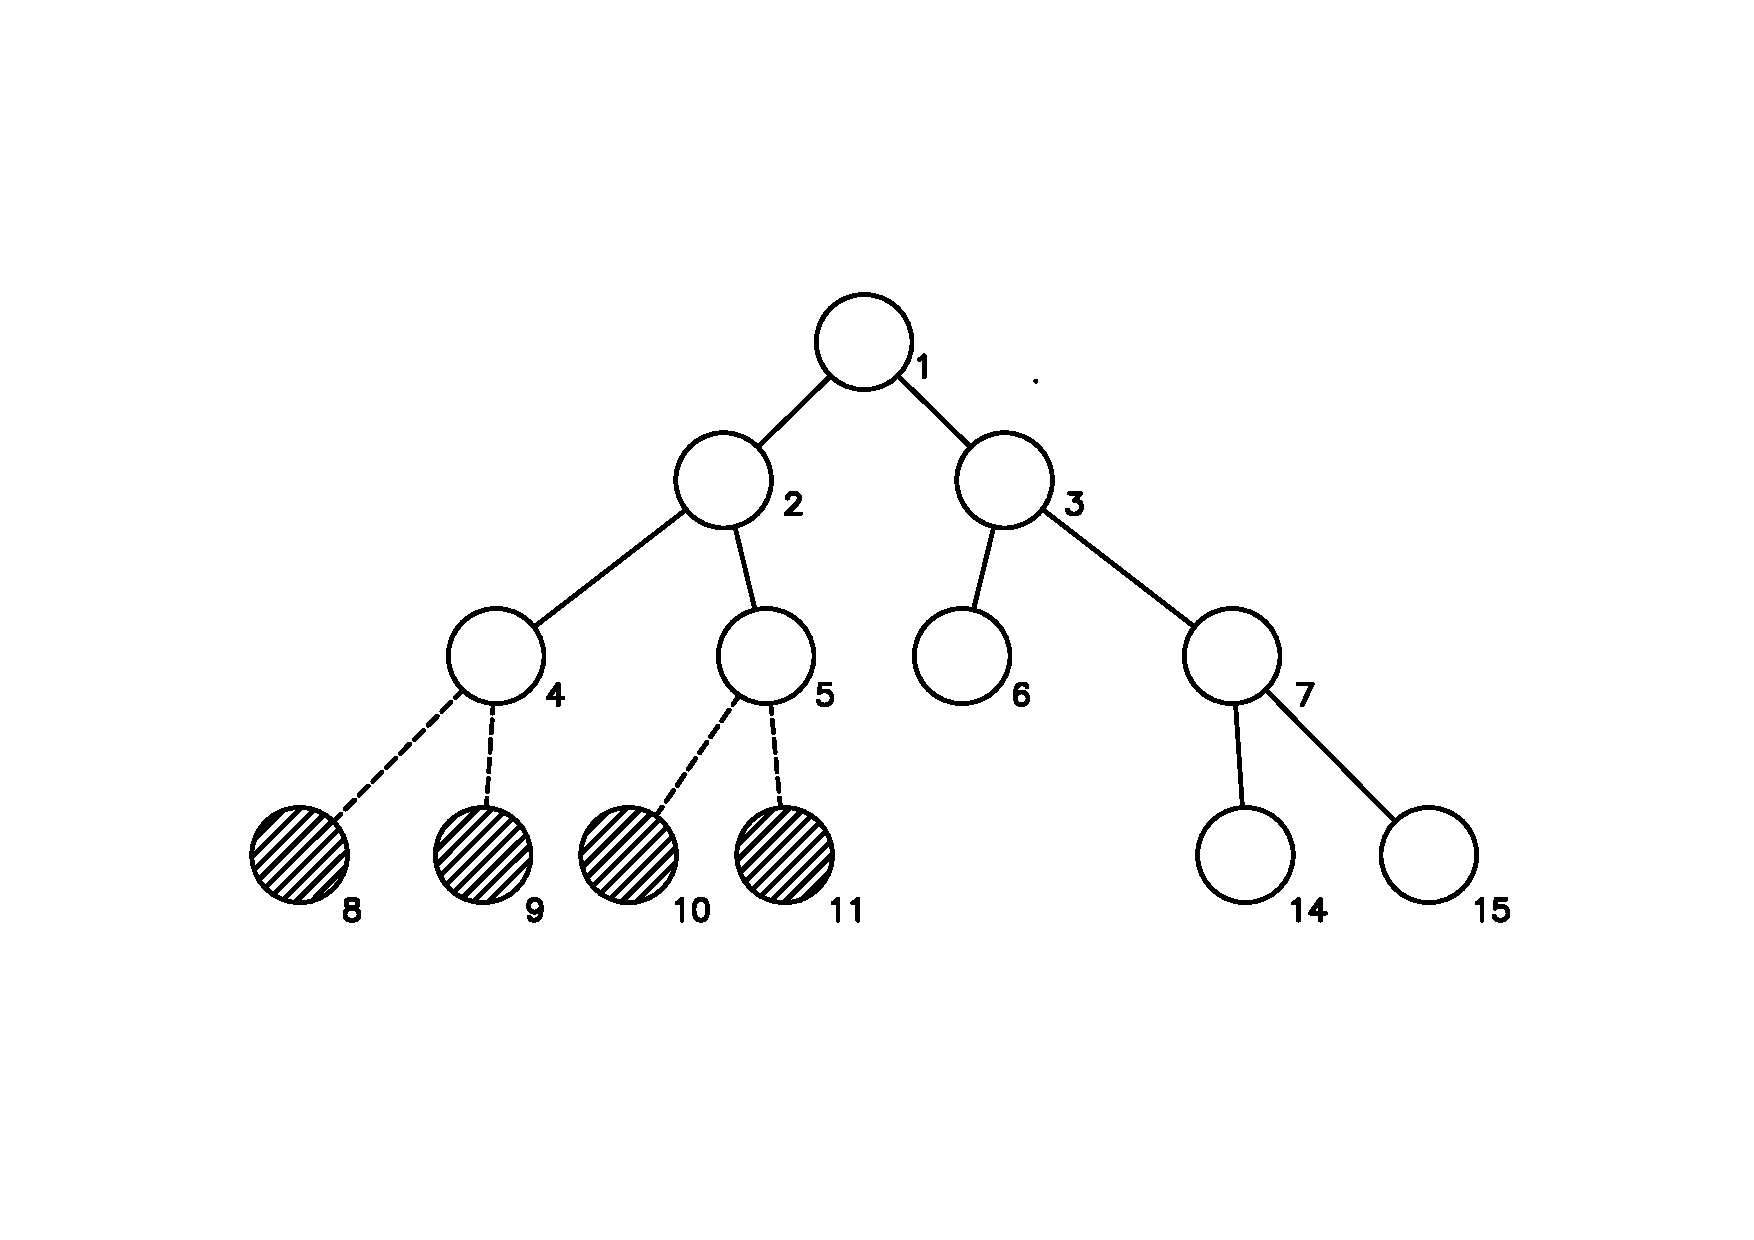
\includegraphics[width=18cm]{figuras/fig1.pdf}
\caption{\label{fig:fig1}Pior caso para $n = 5$.}
\end{figure}

Por se tratar de uma operação onde se deseja encontrar o mínimo, é necessário que haja um número neutro na operação e, neste caso, trata-se de um número fora do universo aqui discutido, ou seja, infinito.
Exemplo: Tendo uma idade qualquer, 42, $min(42, INF) = min(INF, 42) = 42$ e isso é verdade para qualquer número dentro deste universo (idades - 0 - 150 anos).

Aqui, declaramos um vetor de tamanho igual a quatro vezes o número de elementos
do conjunto original, isso se dá pelo seguinte:

A lista original mapeia diretamente para as folhas da árvore, portanto o número de folhas é pelo menos o número de elementos da lista de dados. Uma lista com $2^x$ elementos, gera uma árvore com pelo menos $2^x$ folhas, ou seja, uma árvore com $2^{(x+1)} - 1$ elementos, um vez que a árvore de segmentos é uma árvore binária perfeita. Porém, poderemos ter folhas inúteis no caso em que o tamanho da lista não for uma potência de $2$. No pior caso será uma lista de tamanho $2^x + 1$, onde teremos $2N$ folhas pois temos que arredondar para a próxima potência de $2$. Dessa forma uma árvore binária perfeita com $2N$ folhas terá aproximadamente $4N$ nós no total.

Um exemplo do pior caso está na figura~\ref{fig:fig1}.

Como visto no capítulo anterior, vamos implementar as três principais funções
dessa estrutura: construção, atualização e pergunta de forma recursiva. Por fim, trataremos da união dos nós.

\section{Construção}
Tendo em vista todo o explanado acima, segue a construção da árvore de segmentos, haja vista que desejamos popular o vetor.

\begin{lstlisting}
void build(int node = 1, int l = 0, int r = n) {
    if (l + 1 == r) {
        segtree[node] = v[l];
        return;
    }
    int mid = (l + r)/2;
    build(2*node, l, mid);
    build(2*node+1, mid, r);
    segtree[node] = join(segtree[2*node], segtree[2*node+1]);
}
\end{lstlisting}
Esta função deve ser chamado logo após a leitura da lista de idades, aqui representada por $v$. 
Para simular, vamos supor a seguinte lista apresentada:
$$(5, 3, 11, 7, 1)$$
A ideia do algorítimo é iniciar pelo nó que representará a árvore em sua totalidade e chamar recursivamente para as metades de, aproximadamente, mesmo tamanho, sendo o caso base quando só há um sub elemento na sub árvore para qual a função está sendo chamada.

É importante notar que para esta implementação estamos utilizando uma convenção de intervalos fechados à esquerda e abertos à direita ($[)$).

Simularemos, então a construção da árvore para a lista apresentada acima:
 
A primeira chamada $l = 0$ e $r = n$.
Este intervalo tem tamanho $5$ e portanto calcularemos a sua metade, $mid = 2$ o que resulta em duas chamadas, uma para o nó $2$, com $l = 0$ e $r = 2$ e outra para o nó $3$ com $l = 2$ e $r = 5$.

A chamada para o nó $2$ se desdobrará em duas chamadas para os nós $4$ e $5$, ambos com intervalos de tamanho $1$ que, portanto, retornarão seus elementos na lista de idades, $5$ e $3$, o que resulta neste sendo valorado em $3$ que é o $min(5, 3)$.

Até o momento temos a seguinte situação:

Lista de idades: $$(5, 3, 11, 7, 1)$$
Árvore de segmento: $$(-, -, 3, -, 5, 3)$$

Vamos continuar com a chamada para o nó $3$. Esta por sua vez será subdividida em duas chamadas, para o nó $6$ com $l = 2$ e $r = 3$ e para o nó $7$ com $l = 3$ e $r = 5$. O nó $6$ retornará a casa $2$ da lista de idades, por ter tamanho unitário. Já a chamada para o nó $7$ terá de ser subdividida uma vez mais para os elementos $3$ e $4$ da lista, $7$ e $1$ (nós $14$ e $15$). Com isso o nó $7$ resolve para $1$ e o nó $3$ para $1$ também pois $1 = min(1, 11)$.

Lista de idades: $$(5, 3, 11, 7, 1)$$
Árvore de segmento: $$(-, 1, 3, 1, 5, 3, 11, 1, -, -, -, -, -, -, 7, 1)$$

Árvore criada para essa lista esta na figura~\ref{fig:fig2}.
\begin{figure}[htb]
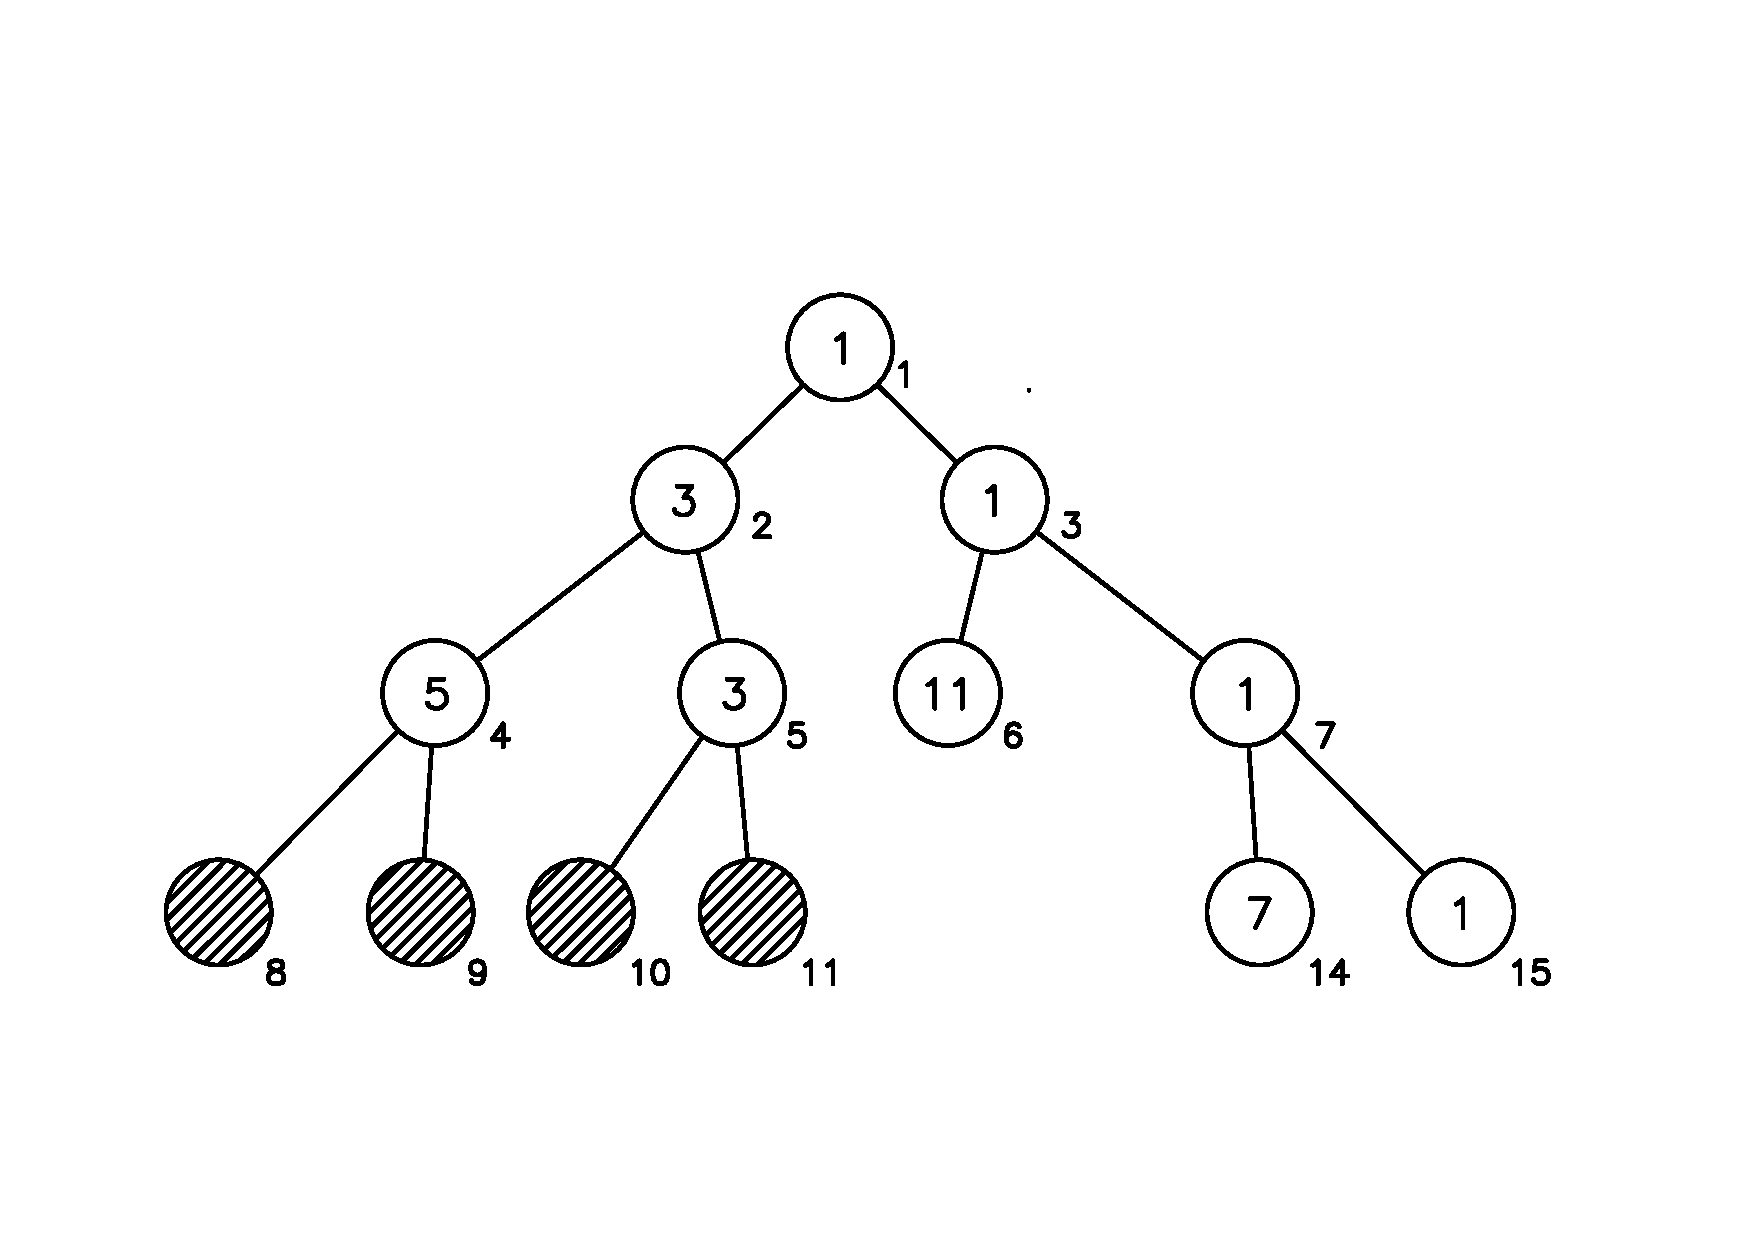
\includegraphics[width=18cm]{figuras/fig2.pdf}
\caption{\label{fig:fig2}Representação dessa árvore.}
\end{figure}

Com isso a árvore de segmentos está construída. Importante notar que a casa $0$ da árvore permanece sem uso para o essa implementação da estrutura.

Como verificado, cada elemento da lista de idades e cada casa do vetor que representa a árvore de segmentos é acessado somente uma vez portanto a construção da árvore tem gasto de tempo de ordem linear no tamanho da lista de idades $O(N)$.

\section{Atualização}
Explanado o campo da construção da estrutura da árvore de segmentos, passamos a apreciar sua atualização.

\begin{lstlisting}
void update(int pos, int value, int node = 1, int l = 0, int r = n) {
    if (l + 1 == r) {
        v[pos] = value;
        return;
    }
    int mid = (l + r)/2;
    if (pos < mid)
        update(pos, value, 2*node, l, mid);
    else update(pos, value, 2*node+1, mid, r);
    segtree[node] = join(segtree[2*node], segtree[2*node+1]);
}
\end{lstlisting}

Sempre que houver necessidade em atualizar alguma das idades da lista de idades, essa função deverá ser chamada.

Suponhamos que gostaríamos de atualizar a 4ª casa da lista em questão, de $1$ para $17$:

Lista original $$(5, 3, 11, 7, 1)$$

Lista atualizada $$(5, 3, 11, 7, 17)$$

Esta atualização seria encapsulada da seguinte forma:$update(4, 17)$.

Vamos, então, simular esta atualização. A chamada é inicializada com $l = 0$ e $r = 5$ e com isso $mid = 2$. 

Como gostaríamos de atualizar a casa $4$ seguiremos com a chamada para o nó $3$, $(4, 17, 3, 2, 5)$, ou seja, não olharemos para o nó $2$, nem para nenhum nó contido em sua sub árvore.

Uma vez no nó $3$, $mid = 3$, logo seguiremos para o nó $7$, pois $4 \geq 3$.

Por ordem, iremos para o nó $15$, pois $4 \geq 4$. Este nó representa um intervalo unitário e, exatamente, a folha que gostaríamos de atualizar que resultará na atualização de todos os nós decorrentes deste, pelo caminho, até a raiz, que, neste caso, serão os nós $15, 7, 3, 1$, fazendo com que a árvore fique da seguinte forma:

Lista de idades: $$(5, 3, 11, 7, 17)$$
Árvore de segmento: $$(-, 3, 3, 7, 5, 3, 11, 7, -, -, -, -, -, -, 7, 17)$$

Árvore depois da atualização esta na figura~\ref{fig:fig3}.
\begin{figure}[htb]
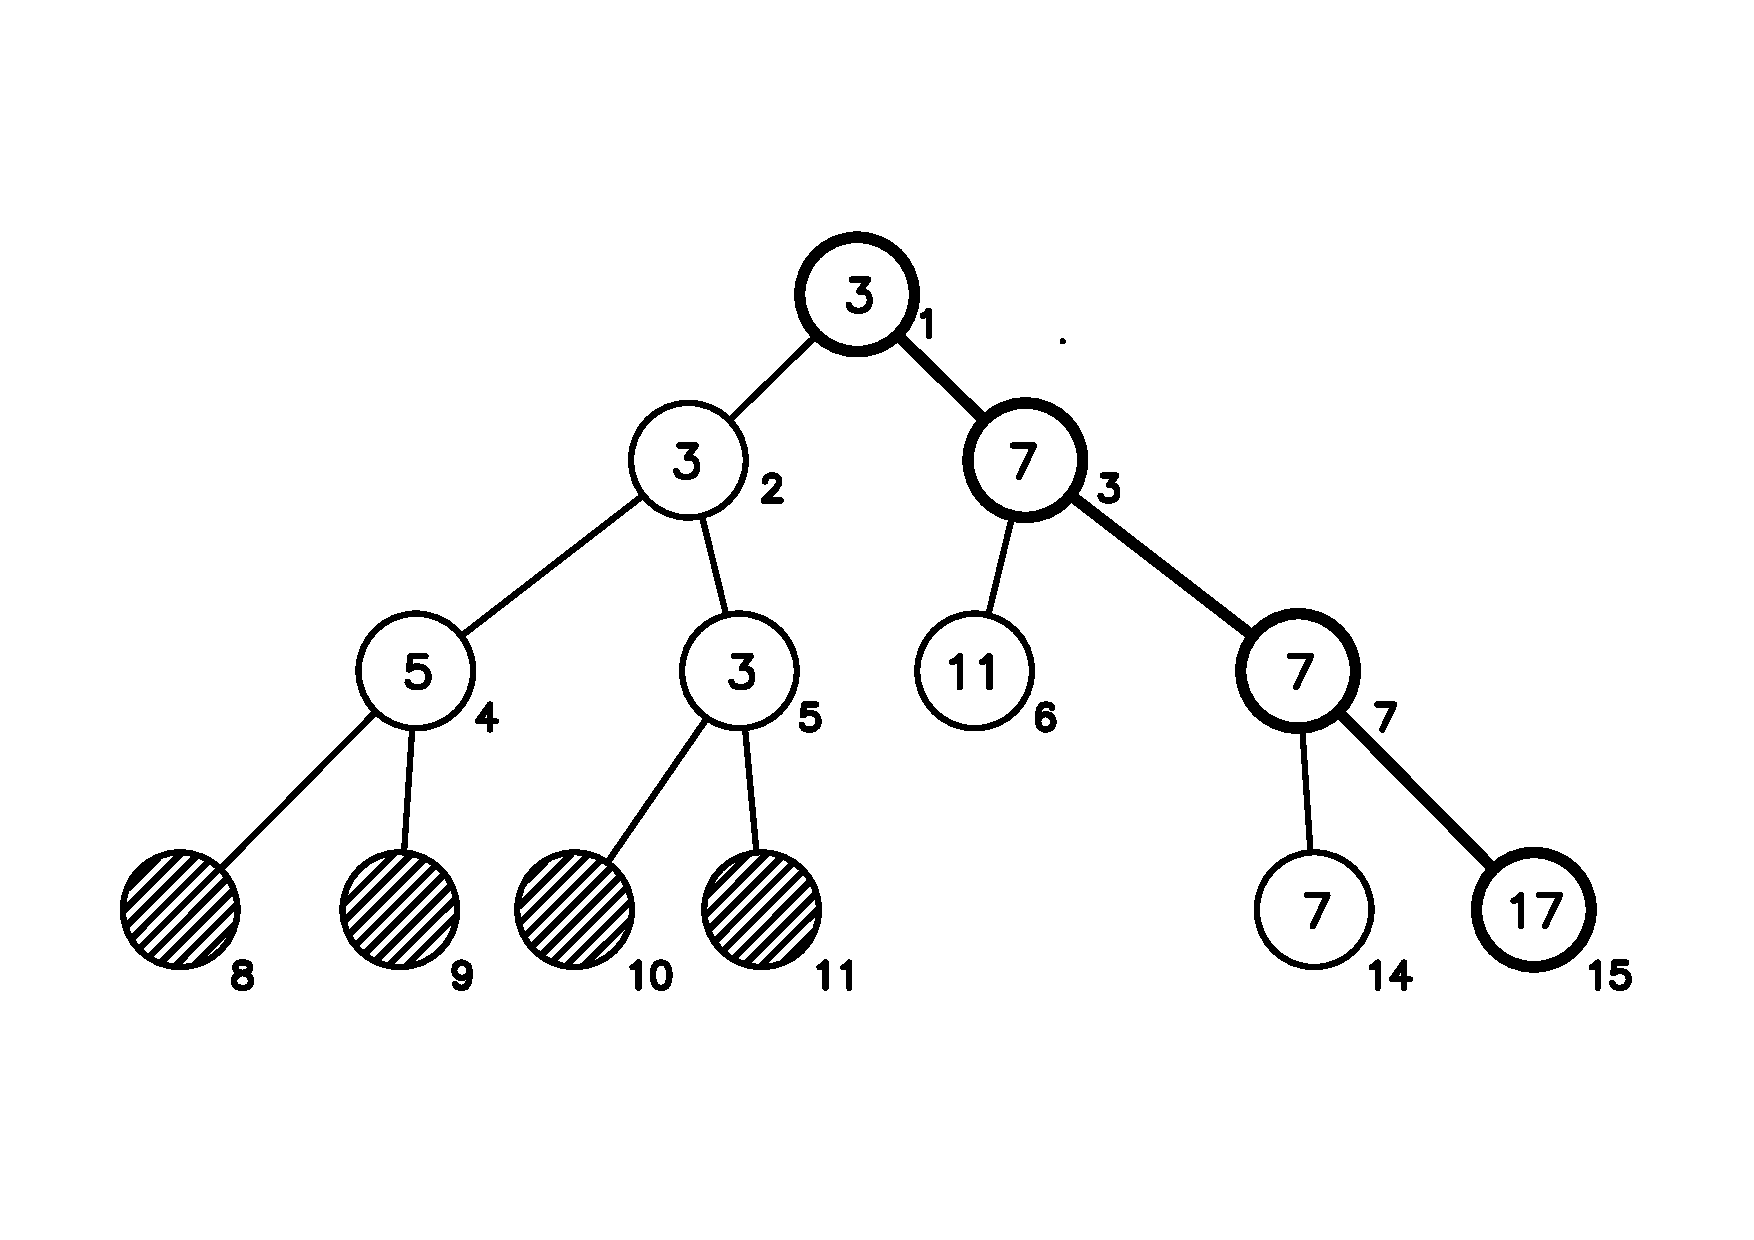
\includegraphics[width=18cm]{figuras/fig3.pdf}
\caption{\label{fig:fig}Árvore atualizada.}
\end{figure}

Como podemos perceber essa função gasta tempo proporcional aos nós que precisam ser inspecionados durante a atualização, que são sempre algum caminho de alguma folha até a raiz. Como a árvore de segmento é uma árvore binária, sua altura é da ordem de $O(\log N)$.

\section{Pergunta}
Conforme vimos desde o início do capítulo, nosso objetivo é encontrar o valor mínimo dado um determinado intervalo (ou vários) utilizando uma estrutura de dados denominada de árvore de segmentos.
Para tanto, já delineamos a definição dos dados a serem analisados apresentando aspectos da construção da árvore de segmentos e sua atualização.
Partiremos, agora, para as perguntas possíveis dados os intervalos e a lista de dados apresentada.

\begin{lstlisting}
int query(int x, int y, int node = 1, int l = 0, int r = n) {
    if (x >= r || y <= l) return NEUTRAL;
    if (x <= l && y >= r) return segtree[node];
    int mid = (l + r)/2;
    return join(query(x, y, 2*node, l, mid), query(x, y, 2*node+1, mid, r));
}
\end{lstlisting}

Suponha que desejamos saber o índice do habitante mais novo entre os habitantes de índices $2$ e $4$ da lista original. Para isso chamamos $query(2, 5)$. 
Lista de idades: $$(5, 3, 11, 7, 1)$$
Por inspeção sabemos que a resposta é o habitante da casa número $4$, de idade $1$.

Vamos simular o algoritmo que determina essa resposta, ou seja, partiremos da chamada $query(2, 5)$. Como o intervalo de interesse $[2, 5)$ não está totalmente disjunto, primeiro caso base, nem contém totalmente o intervalo que estamos observando, segundo caso base, calcularemos a resposta para os dois sub intervalos, $[0, 2)$ e $[2, 5)$.

O intervalo de interesse continua sendo $[2, 5)$, e nesse caso a primeira chamada recursiva está totalmente disjunta e portanto retorna o valor neutro. Já a segunda chamada está totalmente contido e portanto retorna o valor do nó $3$, que representa exatamente esse intervalo, $[2, 5)$. Com isso o retorno de $query(2, 5)$ é $min(INF, 1) = 1$.

A operação supra mencionada também passa por um caminho entre uma folha e a raiz e portanto tem gasto de tempo proporcional a altura da árvore $O(\log N)$.


\section{União de dois nós}
Essa operação pode parecer redundante nesse caso, porém uma vez que um nó 
guardar mais informações faz sentido existir uma função para resolver a 
união de dois nós. Dessa forma podemos obter com a mesma implementação uma 
árvore de segmentos de mínimo, máximo ou máximo divisor comum entre outros 
mudando somente a função de união e a constante neutra da sessão anterior.
\begin{lstlisting}
int join(int a, int b) {
    return min(a, b);
}
\end{lstlisting}
De acordo com o objetivo, no caso em questão, gostaríamos apenas de saber o menor valor do intervalo, logo, a operação de união de dois nós se resume a devolver o mínimo entre eles.

\section{Variações de árvores de segmento ordinárias}
De acordo com tudo que foi discutido até este ponto da pesquisa, já foi possível compreender que é possível implementar variações, que façam com que a estrutura suporte operações diferentes. É o que veremos a seguir.

\subsection{Máximo}
\begin{lstlisting}
const int NEUTRAL = -INF;
int join(int a, int b) {
    return max(a, b);
}
\end{lstlisting}

Nesse caso queremos retornar o maior elemento do intervalo, e para isso basta que a operação de união dos nós se resuma a retornar o máximo entre os elementos e que o elemento neutro seja o infinito negativo, uma vez que $max(-INF, 42) = max(42, -INF) = 42$.

\subsection{Máximo divisor comum}
\begin{lstlisting}
const int NEUTRAL = 0;
int join(int a, int b) {
    return __gcd(a, b);
}
\end{lstlisting}
Nesse caso queremos retornar o máximo divisor comum dos elementos do intervalo, e para isso basta que a operação de união dos nós se resuma a retornar o máximo divisor comum entre os elementos e que o elemento neutro seja o $0$, uma vez que $gcd(0, 42) = max(42, 0) = 42$.
